\documentclass[]{rsuqbeamernew}


\title[]{Distributed computing in UQLab\\with the HPC Dispatcher module}

\author[D. Wicaksono]{Damar Wicaksono}
\institute[RSUQ, ETH Z\"urich]{Chair of Risk, Safety and Uncertainty 
Quantification -- ETH Z\"urich}

\date[09.05.2019]

\graphicspath{{Figures/}}
\usepackage{caption}
\usepackage{listings}
\usepackage{tikz}
\usepackage{pifont}
\usepackage{booktabs}% http://ctan.org/pkg/booktabs
\usepackage{xcolor}
\definecolor{myviolet}{RGB}{140,92,180}
\newcommand{\tabitem}{~~\llap{\textbullet}~~}
%\def\checkmark{\tikz\fill[scale=0.4](0,.35) -- (.25,0) -- (1,.7) -- (.25,.15) -- cycle;}

\lstset{
  basicstyle=\ttfamily,
  escapeinside=||
}

\definecolor{codegreen}{rgb}{0,0.6,0}
\definecolor{codegray}{rgb}{0.5,0.5,0.5}
\definecolor{codepurple}{rgb}{0.58,0,0.82}
\definecolor{backcolour}{rgb}{0.95,0.95,0.92}

\lstdefinestyle{mystyle}{
    backgroundcolor=\color{backcolour},   
    commentstyle=\color{codegreen},
    keywordstyle=\color{magenta},
    numberstyle=\tiny\color{codegray},
    stringstyle=\color{codepurple},
    basicstyle=\ttfamily\footnotesize,
    breakatwhitespace=false,         
    breaklines=true,                 
    captionpos=b,                    
    keepspaces=true,                 
    numbers=left,                    
    numbersep=5pt,                  
    showspaces=false,                
    showstringspaces=false,
    showtabs=false,                  
    tabsize=2
}

\lstset{style=mystyle}


%% Note: the title page will be created automatically

\newsavebox{\mysavebox}

\begin{document}

%===============================================================================

\section{Motivation}

\begin{frame}{Some problems users might have}

\begin{itemize}
  \item Dispatcher module has been updated: asynchronous mode of execution and 
        a \emph{dispatch-and-fetch} workflow
  \item Two dispatcher-aware functions are available:\\
        \mcode{uq_evalModel} and \mcode{uq_map}.
\end{itemize}

\begin{figure}
  \centering
  \includegraphics[width=1.0\linewidth]{./figures/dispatch-and-fetch.pdf}
\end{figure}

\end{frame}


\begin{frame}[fragile]{Distributed computing resources might help...}

\begin{enumerate}
  \setcounter{enumi}{-1}
  \item Create a \textsc{Dispatcher} object
  \item Create a set of configuration options:
\end{enumerate}
\begin{lstlisting}[basicstyle=\scriptsize,numbers=none]
ParamsOpts.Type = 'Metamodel';
ParamsOpts.MetaType = 'Kriging';

ParamsOpts.Trend.Type = {'polynomial'};
ParamsOpts.Trend.Degree = {0,1,2};

ParamsOpts.Corr.Type = {'ellipsoidal', 'separable'};
ParamsOpts.Corr.Family = {'linear', 'exponential', 'gaussian',...
    'matern-3_2','matern-5_2'};
ParamsOpts.Corr.Isotropic = {true, false};

ParamsOpts.EstimMethod = {'CV','ML'};
  
ParamsOpts.Optim.Method = {'BFGS', 'GA', 'HGA', 'CMAES', 'HCMAES'};
  
ParamsOpts.ExpDesign.X = {Xtrain};
ParamsOpts.ExpDesign.Y = {Ytrain};
ParamsOpts.ValidationSet.X = {Xval};
ParamsOpts.ValidationSet.Y = {Yval};

% Create the set, 600 configuration options (struct array)
ParamSets = uq_createParameterSets(ParamsOpts); 
\end{lstlisting}

\end{frame}

\begin{frame}[fragile]{Distributed computing resources might help, but...}

\begin{enumerate}
  \setcounter{enumi}{1}
  \item \emph{Map} the set of configurations options using \mcode{uq_createModel}\\
         and dispatch the calculation to the remote machine:
\begin{lstlisting}[basicstyle=\scriptsize]
uq_map(@uq_createModel, ParamSets, myDispatcher, 'UQLab', true)
\end{lstlisting}
  \item (when finished) \emph{Fetch} all the Kriging objects from the remote machine:
\begin{lstlisting}[basicstyle=\scriptsize]
myModels = uq_fetchResults(myDispatcher)
ans =

  600x1 cell array

    {1x1 uq_model}
    {1x1 uq_model}
    {1x1 uq_model}
    {1x1 uq_model}
    {1x1 uq_model}
    {1x1 uq_model}
    ...
\end{lstlisting}
  \item Analyze the resulting objects (\eg{,} compare LOO and validation errors)
\end{enumerate}

\begin{itemize}
  \item On-going tasks: Documentation writeup and some additional testings
\end{itemize}

\end{frame}

%==============================================================================
\begin{frame}
\frametitle{Distributed computing resources might help, but...}
\begin{block}{Your institution has distributed computing resources, so you:}
\begin{enumerate}
  \item ask/look around how to get an access
  \item get an access (username, password, computing time, storage space)
  \item read the Wiki
  \item are ready for some distributed computing \only<2>{{\altx (right?)}}
\end{enumerate}
\end{block}
\begin{block}{\textbf{EULER}: Large HPC infrastructure of the ETHZ}
\begin{figure}[htbp]
  \includegraphics[width=\textwidth]{./figures/ETH_Zurich_Euler_II_and_I_in_LCA}\\
  {\tiny Credit: Olivier Byrde, ETH Zurich (2015)}
%  \hspace*{15pt}\hbox{\scriptsize Credit:\thinspace{\small\itshape Kathleen Gilje}}
\end{figure}
\end{block}
\end{frame}

%==============================================================================
\begin{frame}
\frametitle<1-8>{Distributed computing in 7 easy steps}
\frametitle<9>{Distributed computing in 7 (\emph{not so}) easy steps}
\begin{columns}
\column{0.4\textwidth}
\setbeamercovered{invisible}
\begin{block}{}
\begin{enumerate}
  \item<2-> Login to the remote machine
  \item<4-> Create an analysis script to run in the remote
  \item<5-> Create a job script
  \item<6-> Submit the job to the queues
  \item<7-> Check the queues until job is finished
  \item<8-> Transfer output files back (\texttt{scp},\texttt{rsync})
  \item<9-> Analyze outputs in the local machine
\end{enumerate}
\end{block}
\column{0.6\textwidth}
\begin{onlyenv}<2-9>
\begin{figure}[htbp]
  \includegraphics<2-3>[width=\textwidth]{./figures/terminal-small.png}
  \includegraphics<4>[width=\textwidth]{./figures/remoteScript.png}
  \includegraphics<5>[width=\textwidth]{./figures/job-script.png}
  \includegraphics<6>[width=\textwidth]{./figures/terminal-small.png}
  \includegraphics<7>[width=\textwidth]{./figures/terminal-small.png}
  \includegraphics<8>[width=\textwidth]{./figures/terminal-small.png}
  \includegraphics<9>[width=\textwidth]{./figures/matlab.png}
\end{figure}
\end{onlyenv}
\setbeamercovered{transparent}
\end{columns}
\end{frame}

%==============================================================================
\begin{frame}
\frametitle{Users vs. Machine}
\begin{figure}[htbp]
  \includegraphics[width=\textwidth]{./figures/dispatcher-gap.pdf}
\end{figure}
\end{frame}
  
%==============================================================================
\begin{frame}
\frametitle{Introducing the HPC \textsc{Dispatcher} module}

\begin{figure}[htbp]
  \includegraphics[width=\textwidth]{./figures/dispatcher-module.pdf}
\end{figure}    

\begin{onlyenv}<1>
\begin{block}{The HPC \textsc{dispatcher} module is an attempt to bridge the gap}
  \begin{itemize}
    \item It allows user to dispatch and retrieve {\altx some computations}
          to remote distributed computing resources
    \item All from a local \textsc{UQLab} session
    \item Emphasis on {\altx some computations}, i.e.,
          certain computations that are relevant in uncertainty quantification (UQ)
          with \textsc{UQLab}
  \end{itemize}
\end{block}
\end{onlyenv}

\setbeamercovered{invisible}
\begin{onlyenv}<2-3>
  \begin{onslide}<2->
  \begin{block}{This presentation is about:}
    \begin{itemize}
      \item The HPC \textsc{dispatcher} module features
      \item Its basic usage and (more advanced) use case
    \end{itemize}
  \end{block}
\end{onslide}

\begin{onslide}<3->
  \begin{block}{...and less about:}
    \begin{itemize}
      \item Distributed computing system
      \item Parallel algorithms and programming
    \end{itemize}
  \end{block}
\end{onslide}
\end{onlyenv}
\setbeamercovered{transparent}

\end{frame}

\begin{frame}[fragile]{Introducing the HPC \textsc{Dispatcher} module}

Watch this slide grow.
\pause
\begin{itemize}
  \item<2-> Hello, World!
  \item<3-> Hello, Mars!
  \item<4-> \textbf<5->{Hello}, Alpha Centauri!
\end{itemize}
  
\end{frame}

\begin{frame}[fragile]
  \frametitle{Including Code}
  \begin{semiverbatim}
  \\begin\{frame\}
  \\frametitle\{Outline\}
  \\tableofcontents
  \\end\{frame\}
  \end{semiverbatim}
\end{frame}

\begin{frame}[fragile]{\texttt{uq\_map}: Mapping function}

\begin{lstlisting}
uq_map(|\textcolor<2>{myviolet}{fun}|,|\textcolor<3>{myviolet}{inputs}|)
\end{lstlisting}
\begin{itemize}
  \item \textcolor<2>{myviolet}{mapping function}
  \item \textcolor<3>{myviolet}{input sequence}
\end{itemize}

\end{frame}



  


\begin{frame}[fragile]{D. Wicaksono: Parametric studies with \mcode{uq_map} (2/2)}

\begin{lstlisting}[basicstyle=\scriptsize,numbers=none]
>> uq_evalModel(myModel,X)

\end{lstlisting}
  
\end{frame}

\begin{frame}[fragile]{D. Wicaksono: Parametric studies with \mcode{uq_map} (2/2)}

\begin{lstlisting}[basicstyle=\scriptsize,numbers=none]
>> uq_evalModel(myModel,X,'HPC')

ans =

     []
\end{lstlisting}

\setbeamercovered{invisible}
\onslide<2->{\emphconc{Whoa}}
\setbeamercovered{transparent}

\end{frame}


\section{\textsc{Dispatcher} in action}

%==============================================================================
\begin{frame}[fragile]
\frametitle<1>{\textsc{Dispatcher} in action: Problem setup}
\frametitle<2->{\textsc{Dispatcher} in action: \textsc{Model} evaluation}

Create a \textsc{Model} object from an \mcode{m}-file:
\begin{lstlisting}[basicstyle=\scriptsize]
ModelOpts.mFile = 'uq_ishigami';

myModel = uq_createModel(ModelOpts);
\end{lstlisting}

\begin{onlyenv}<2-2>
Evaluate the \textsc{Model} on a single input point:
\begin{lstlisting}[basicstyle=\scriptsize,numbers=none]
>> uq_evalModel([0.5*pi 0.5*pi 0.5*pi])

ans =
  
    8.6088
\end{lstlisting}
\end{onlyenv}

\begin{onlyenv}<3->
Let's assume a \textsc{Dispatcher} object has been created ({\altx more on this later }).
Dispatch the same \textsc{Model} evaluation to the remote machine:
\begin{lstlisting}[basicstyle=\scriptsize,numbers=none]
>> uq_evalModel([0.5*pi 0.5*pi 0.5*pi],'HPC')
  
ans =
    
    []
\end{lstlisting}
\end{onlyenv}

\setbeamercovered{invisible}
\onslide<4->{\emphconc{Whoa, what happened?}}
\setbeamercovered{transparent}
  
\end{frame}

%==============================================================================
\begin{frame}[fragile]{\textsc{Dispatcher} in action: \emph{Dispatch} a computation}

\begin{lstlisting}[basicstyle=\scriptsize,numbers=none]
>> uq_evalModel(myModel,X,'HPC')
  
ans =
  
    []
\end{lstlisting}
  
\begin{figure}[htbp]    
  \centering
  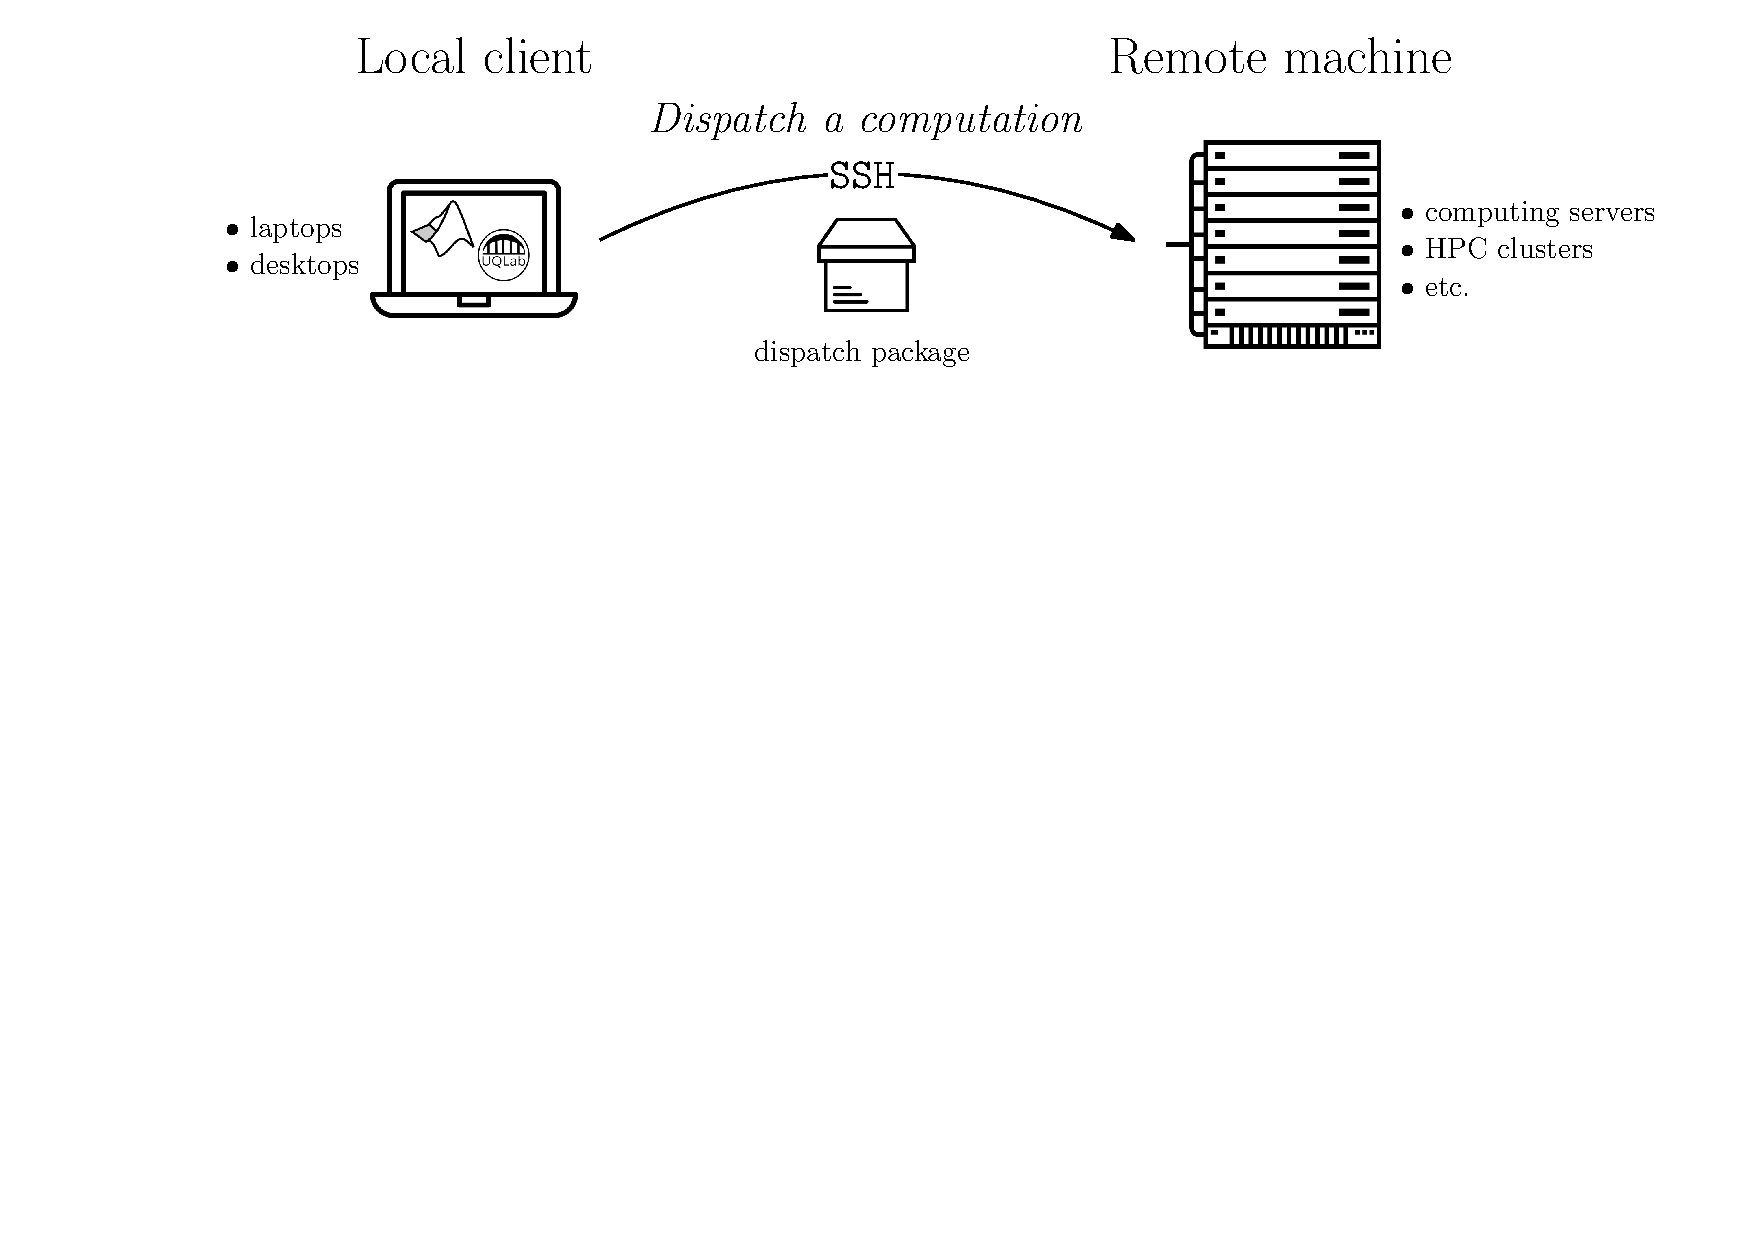
\includegraphics[width= 0.8\textwidth]{./figures/dispatch-and-fetch-dispatch.pdf}
\end{figure}

\end{frame}

%==============================================================================
\begin{frame}[fragile]{Dispatcher in action: asynchronous execution}

\begin{lstlisting}[basicstyle=\scriptsize,numbers=none]
>> uq_evalModel(myModel,X,'HPC')
    
ans =

    []
\end{lstlisting}
    
\begin{figure}[htbp]    
  \centering
  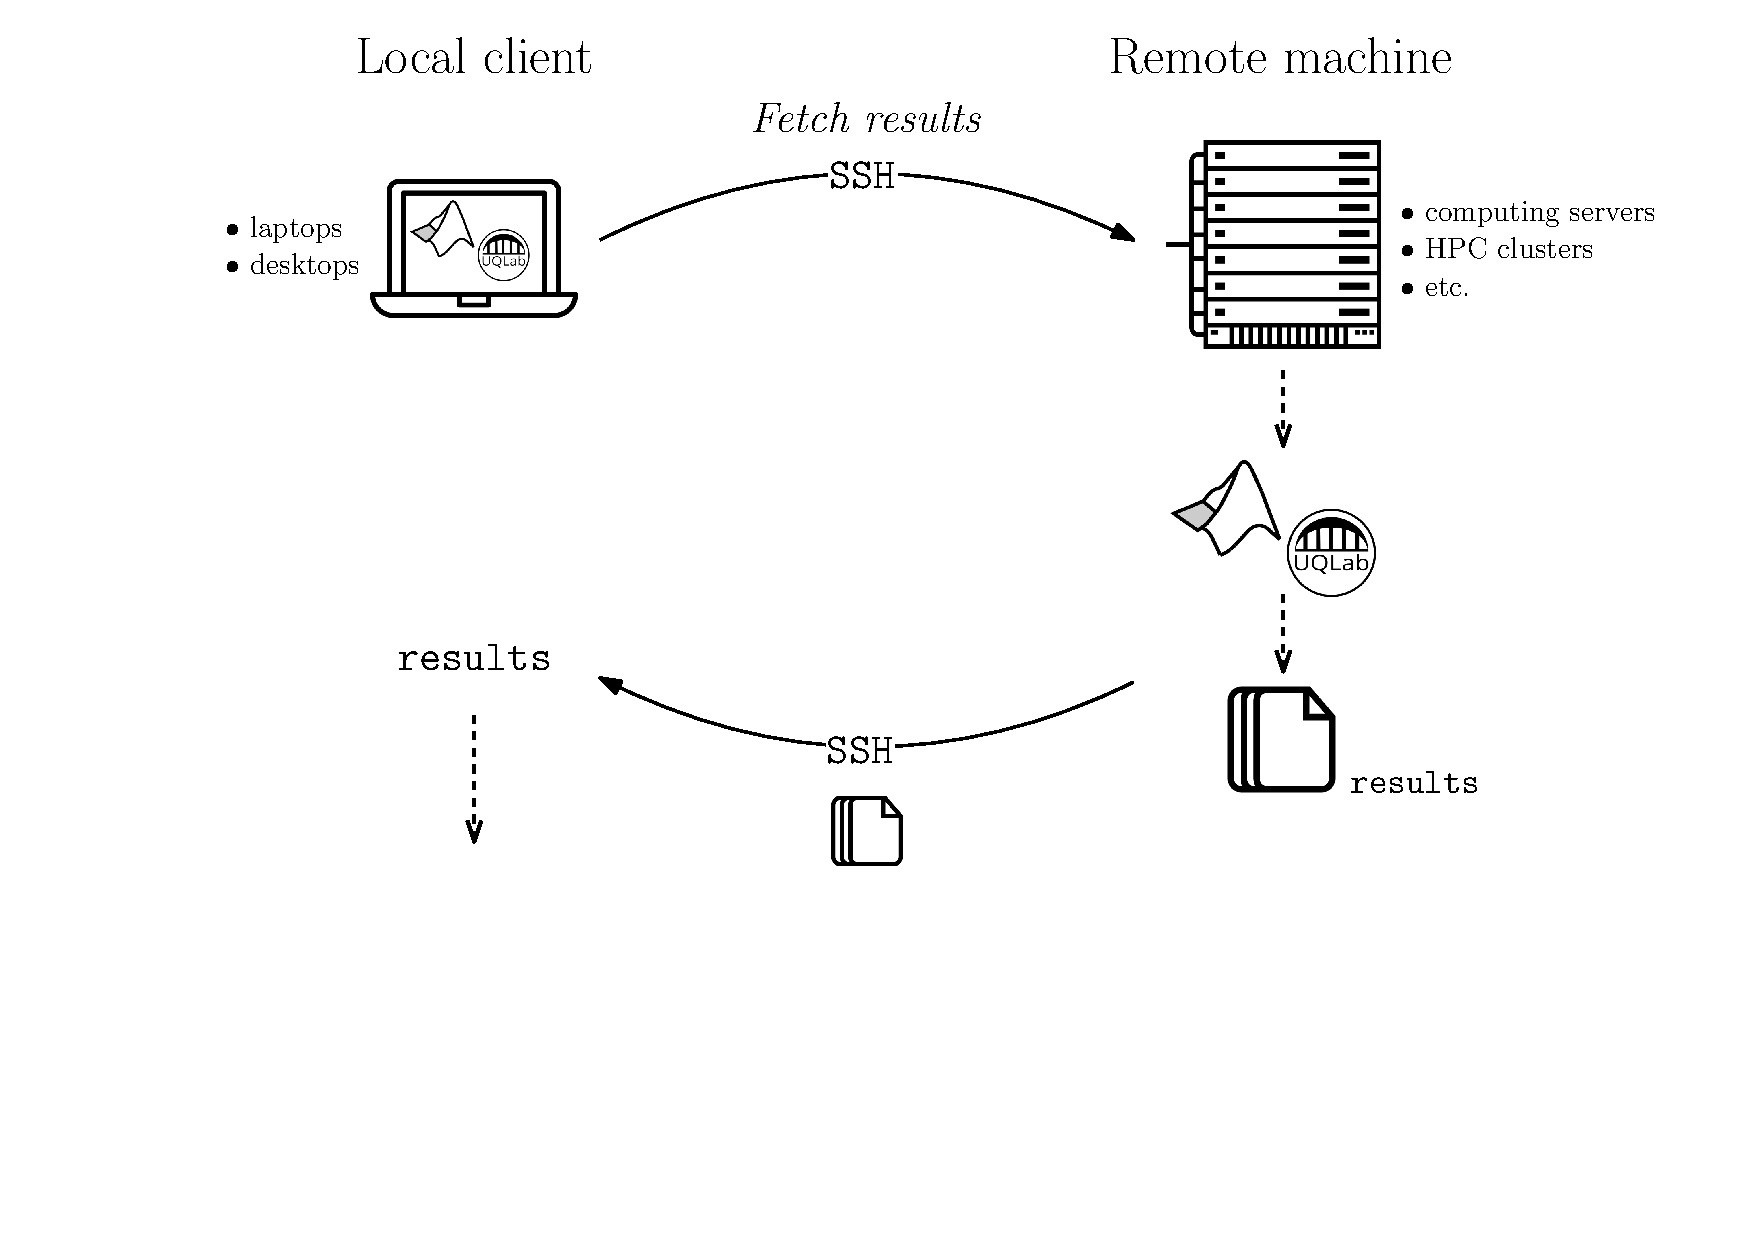
\includegraphics[width= 0.8\textwidth]{./figures/dispatch-and-fetch-fetchResults.pdf}
\end{figure}
  
\end{frame}

%==============================================================================
\begin{frame}[fragile]{Dispatcher in action: asynchronous execution}

  \begin{lstlisting}[basicstyle=\scriptsize,numbers=none]
  >> uq_evalModel(myModel,X,'HPC')
      
  ans =
  
      []
  \end{lstlisting}
      
  \begin{figure}[htbp]    
    \centering
    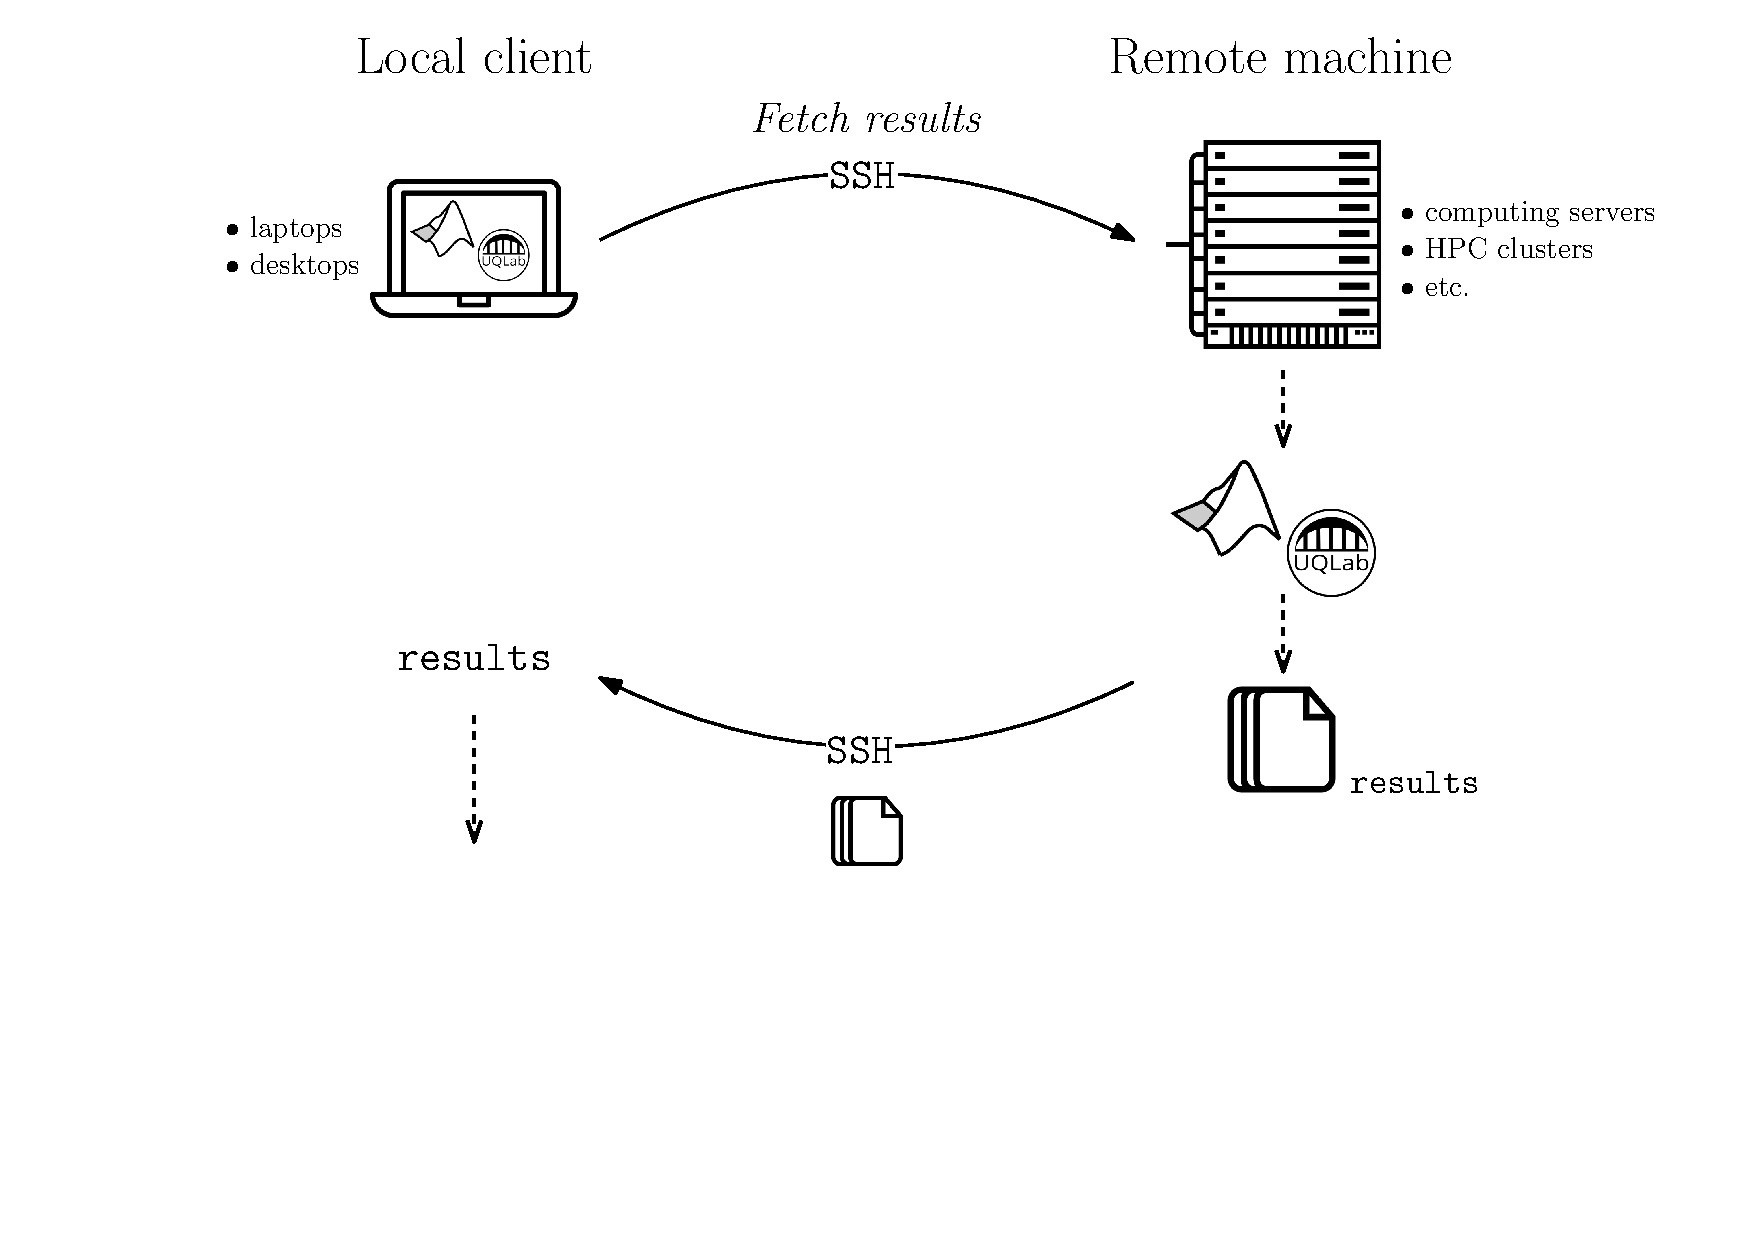
\includegraphics[width= 0.8\textwidth]{./figures/dispatch-and-fetch-fetchResults.pdf}
  \end{figure}
    
  \end{frame}

%==============================================================================
\begin{frame}[fragile]{Dispatcher in action: \emph{Get status}}

\begin{lstlisting}[basicstyle=\scriptsize,numbers=none]
>> uq_getStatus(myDispatcher)
      
ans =

    'running'
\end{lstlisting}
      
\begin{figure}[htbp]    
  \centering
  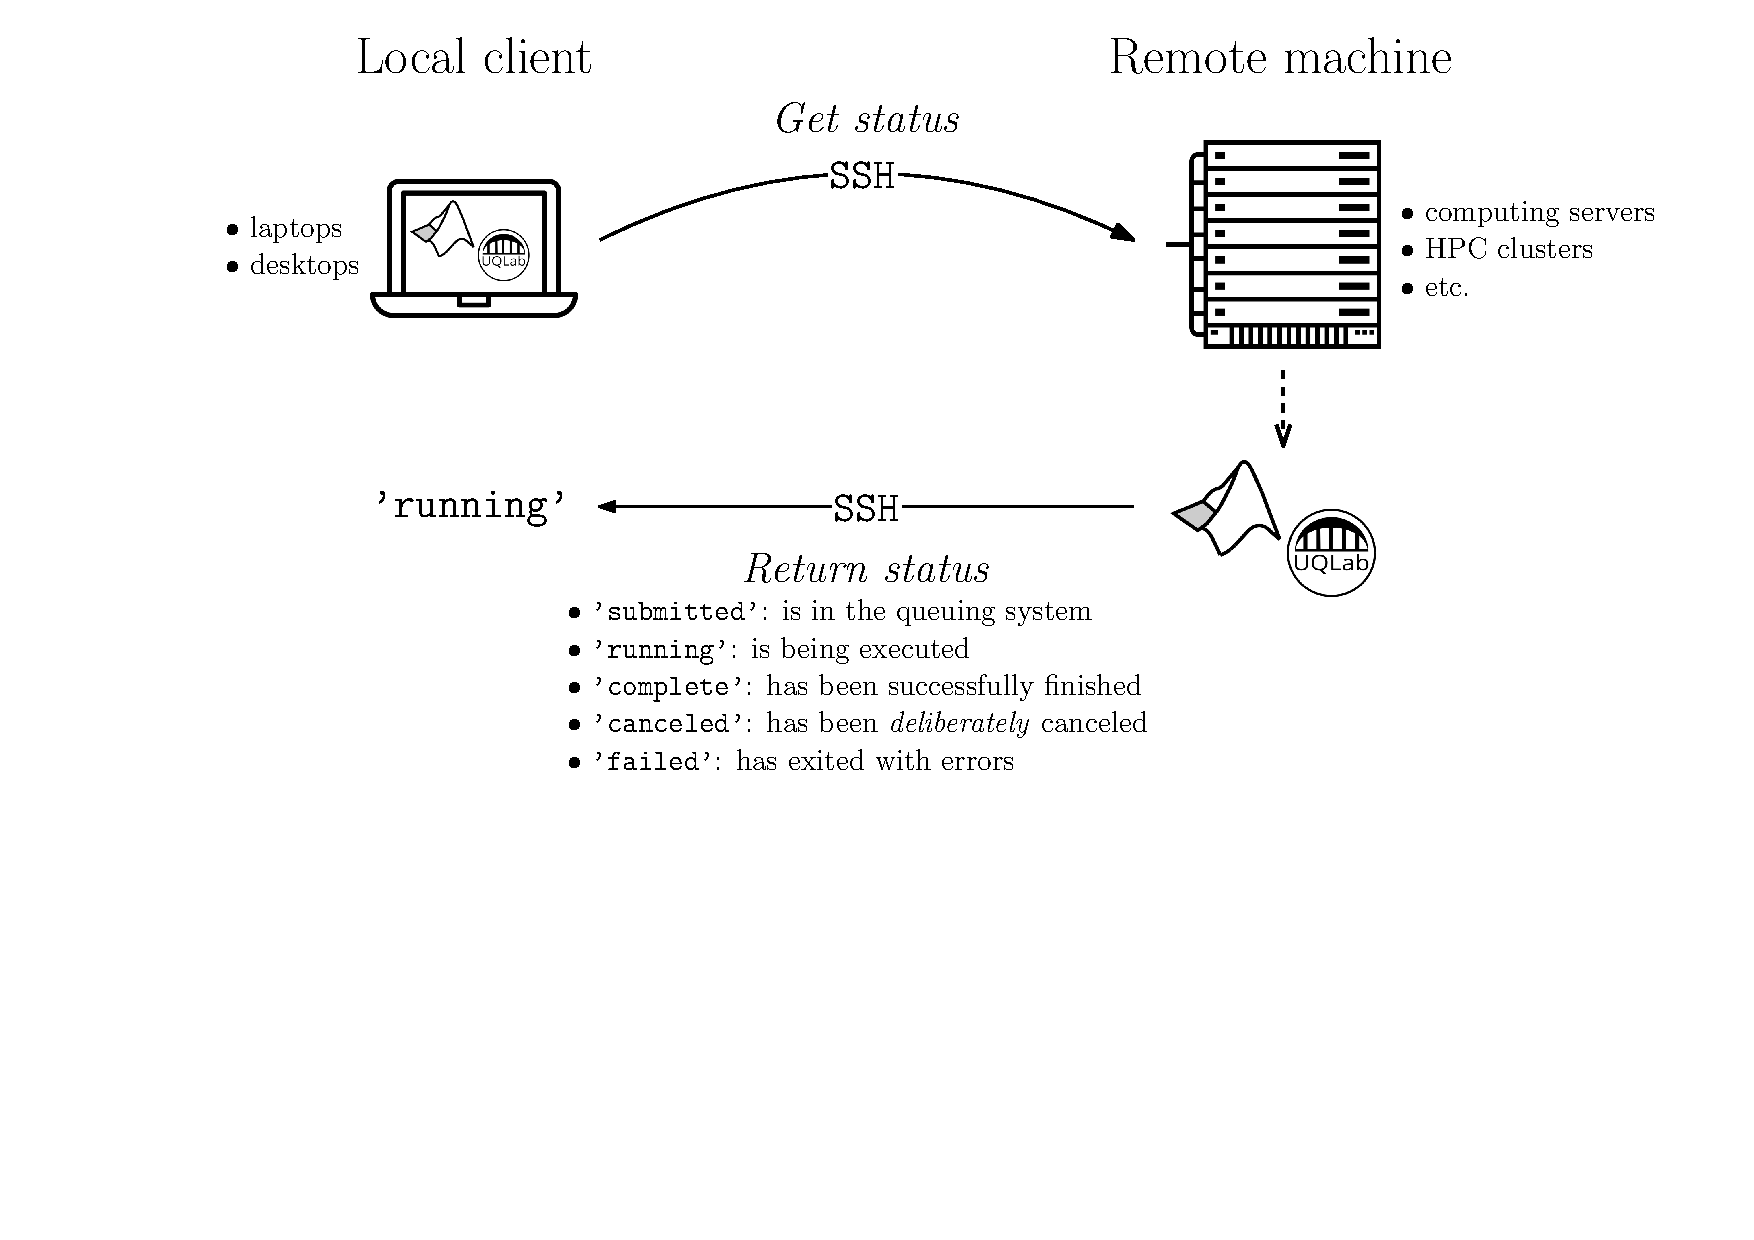
\includegraphics[width= 0.8\textwidth]{./figures/dispatch-and-fetch-getStatus.pdf}
\end{figure}
    
\end{frame}

%==============================================================================
\begin{frame}[fragile]{Dispatcher in action: remote execution is finished}

\begin{lstlisting}[basicstyle=\scriptsize,numbers=none]
>> uq_getStatus(myDispatcher)
      
ans =
  
  'complete'
\end{lstlisting}
      
\begin{figure}[htbp]    
  \centering
  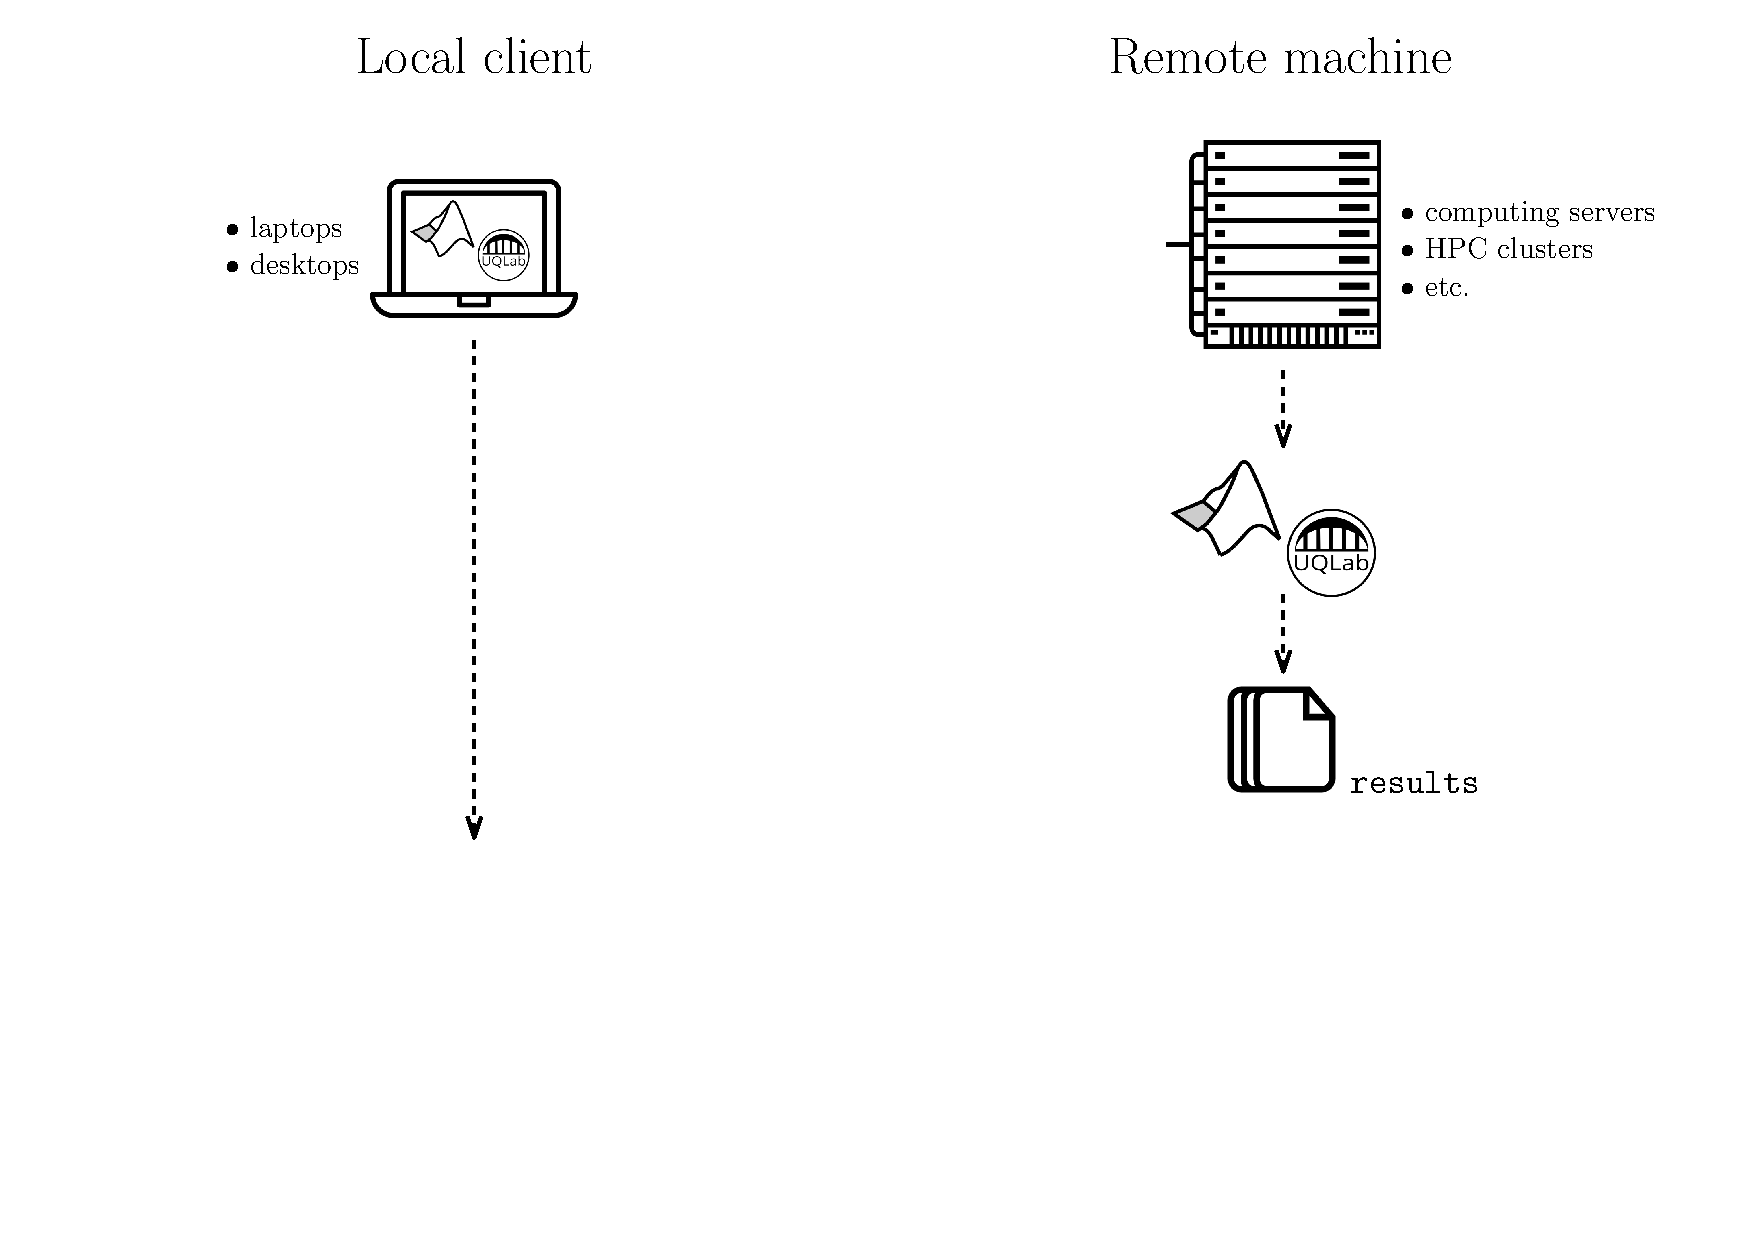
\includegraphics[width= 0.8\textwidth]{./figures/dispatch-and-fetch-completed.pdf}
\end{figure}
    
\end{frame}

%==============================================================================
\begin{frame}[fragile]{Dispatcher in action: \emph{Fetch results}}

\begin{lstlisting}[basicstyle=\scriptsize,numbers=none]
>> results = uq_fetchResults(myDispatcher)

results =

    8.6088
\end{lstlisting}
        
\begin{figure}[htbp]
  \centering
  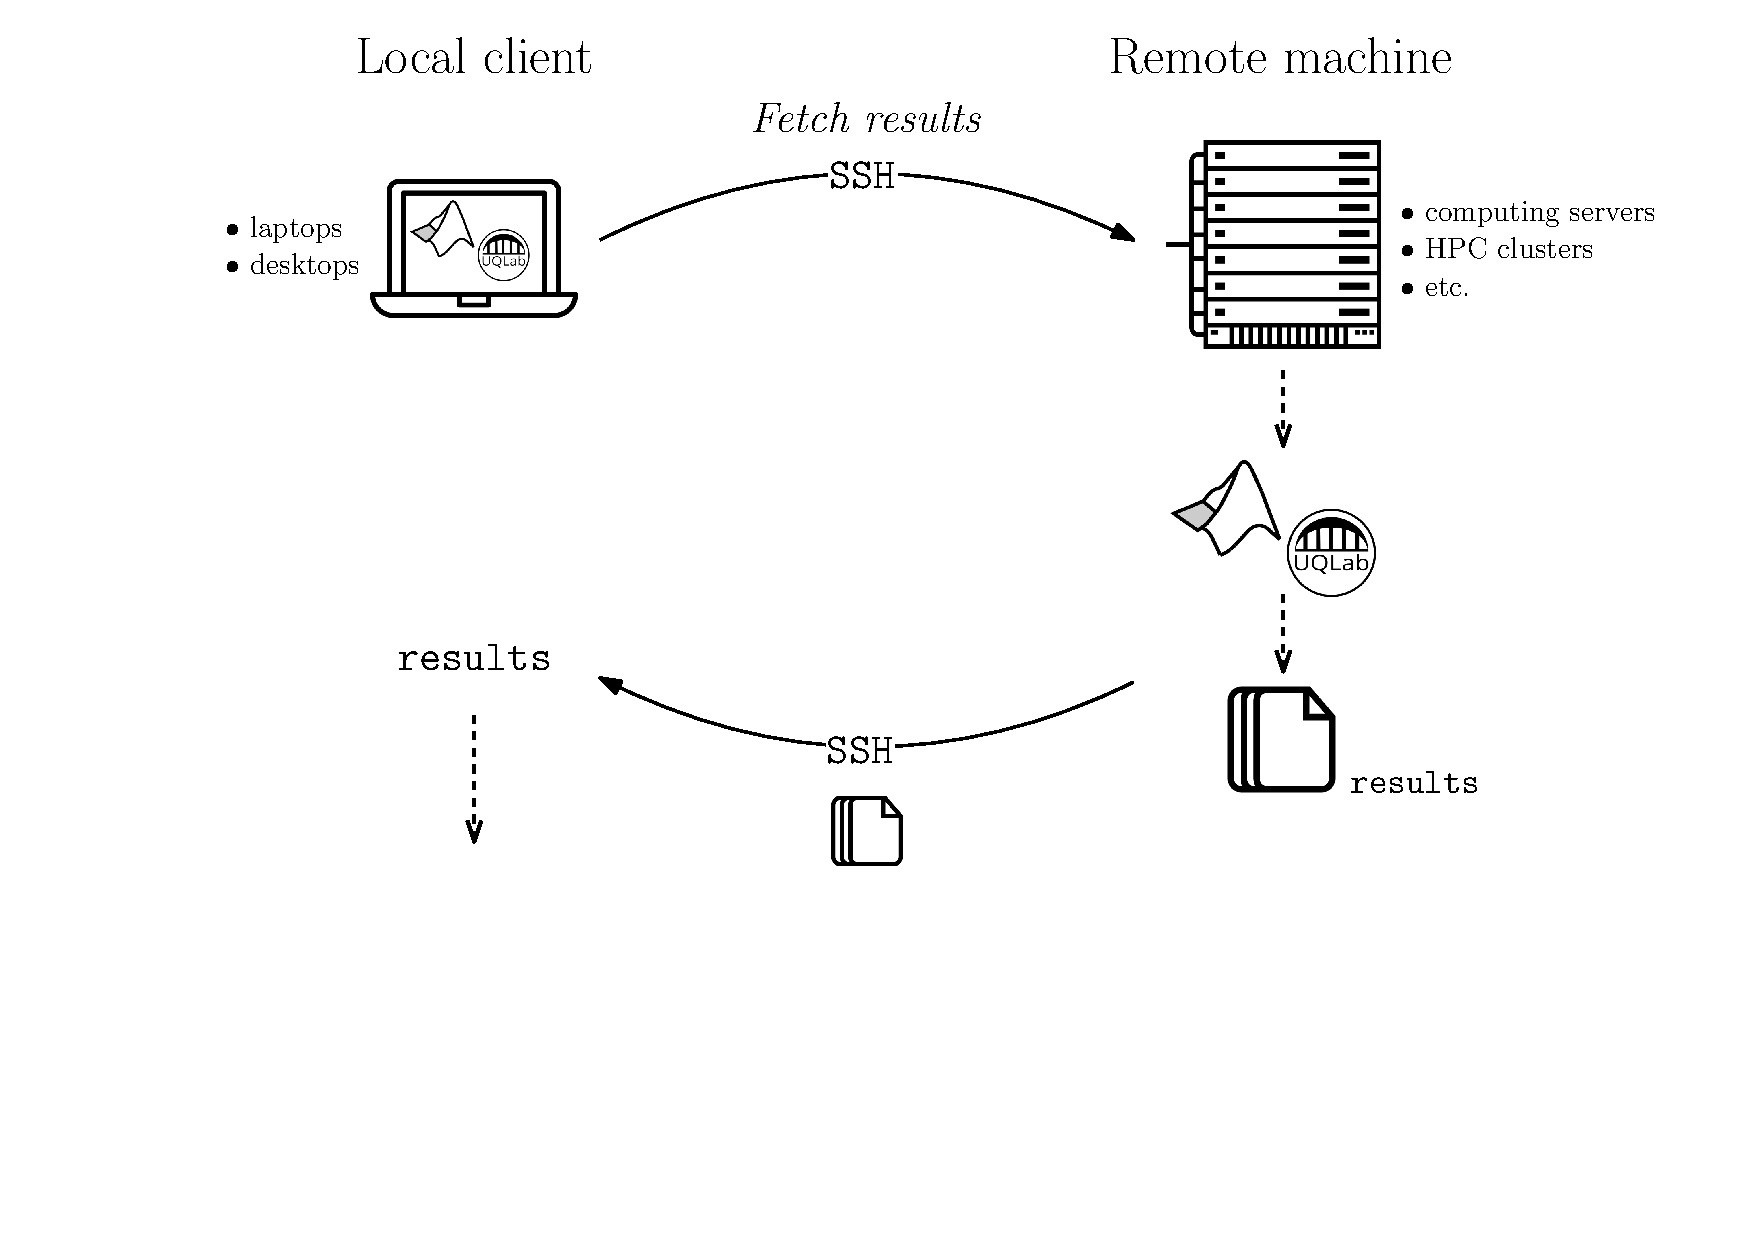
\includegraphics[width= 0.8\textwidth]{./figures/dispatch-and-fetch-fetchResults.pdf}
\end{figure}
      
\end{frame}

%==============================================================================
\begin{frame}[fragile]{Backtrack: Setting up a Dispatcher object}

\onslide<1->{\begin{block}{What you need to set up and use a Dispatcher object}
\begin{itemize}
  \item An access to a remote machine; it must run a Linux OS and has an MPI implementation
  \item A directory with write access permission in the remote machine
  \item A passwordless SSH connection to the remote machine
  \item A profile file that stores required information about the remote machine 
\end{itemize}
\end{block}}

\end{frame}

%==============================================================================
\begin{frame}[fragile]{Backtrack: Setting up a Dispatcher object}

\begin{block}{What you need to set up and use a Dispatcher object}
\begin{itemize}
  \item An access to a remote machine; it must run a Linux OS and has an MPI implementation
  \item A directory with write access permission in the remote machine
  \item A passwordless SSH connection to the remote machine
  \item A profile file that stores required information about the remote machine 
\end{itemize}
\end{block}
  
An example of a (minimum) remote machine profile file (\texttt{myProfile.m}):
\begin{lstlisting}[basicstyle=\scriptsize]
Hostname = 'euler.ethz.ch';
Username = 'wdamar';
PrivateKey = '~/.ssh/id_rsa_dispatcher';
RemoteFolder = '/home/wdamar/temp';
\end{lstlisting}
  
\end{frame}

%==============================================================================
\begin{frame}[fragile]{Backtrack: Setting up a Dispatcher object}

\only<1>{\begin{block}{What you need to set up and use a \textsc{Dispatcher} object}
\begin{itemize}
  \item An access to a remote machine; it must run a Linux OS and has an MPI implementation
  \item A directory with write access permission in the remote machine
  \item A passwordless SSH connection to the remote machine
  \item A profile file that stores required information about the remote machine 
\end{itemize}
\end{block}}
  
\only<2>{\emphconc{No \textsc{MATLAB}/\textsc{UQLab} in the remote machine is required
for \textsc{UQLink} model evaluation}}

An example of a (minimum) remote machine profile file (\texttt{myProfile.m}):
\begin{lstlisting}[basicstyle=\scriptsize]
Hostname = 'euler.ethz.ch';
Username = 'wdamar';
PrivateKey = '~/home/wdamar/.ssh/id_rsa_dispatcher';
RemoteFolder = '/home/wdamar/temp';
\end{lstlisting}
  
In a \textsc{UQLab} session:
\begin{lstlisting}[basicstyle=\scriptsize,numbers=none]
DispatcherOpts.Profile = 'myProfile';
  
myDispatcher = uq_createDispatcher(DispatcherOpts);
\end{lstlisting}
  
\end{frame}

%==============================================================================
\begin{frame}[fragile]{\textsc{UQLink} \textsc{model} evaluation in a cloud cluster}

An example of distributed computing on a ({\altx not} high performance) cluster 
\begin{itemize}
  \item Input files are created locally
  \item 3rd-party code is executed on the remote (must be installed there) 
  \item Output files are parsed locally
\end{itemize}

\begin{figure}[htbp]
  \centering
  \includegraphics[width=\textwidth]{./figures/dispatch-droplet.pdf}
\end{figure}
    
\end{frame}

%==============================================================================
\begin{frame}[fragile]{Backtrack: Setting up a \textsc{Dispatcher} object}

Additional settings in the remote profile file:
\begin{itemize}
  \item For generic \textsc{UQLab} computations, you'd need \textsc{MATLAB} and \textsc{UQLab}:
\begin{lstlisting}[basicstyle=\scriptsize,numbers=none]
...
MATLABCommand = '/usr/local/bin/matlab';
RemoteUQLabPath = '~/uqlab';
\end{lstlisting}

  \item The remote machine might also employ a \emph{job scheduler}:
\begin{lstlisting}[basicstyle=\scriptsize,numbers=none]
...
Scheduler = 'slurm';  % or 'lsf', 'pbs', 'torque'
\end{lstlisting}
   
  \item It might also employ a \emph{module} system to load software and set up their environment:
\begin{lstlisting}[basicstyle=\scriptsize,numbers=none]
...
EnvSetup = 'module load open_mpi';    % only on the login node
PrevCommands = 'module load matlab';  % aso on the compute nodes
\end{lstlisting}

  \item And some other settings (e.g., custom scheduler, MPI settings);
  see the Reference List of the \textsc{Dispatcher} module user manual.
\end{itemize}

\end{frame}

\section{\texttt{uq\_map}}
%==============================================================================
\begin{frame}[fragile]{Dispatching generic functions}

\textbf{\emphconc{How about dispatching an evaluation of a generic function?}}

\end{frame}

%==============================================================================
\begin{frame}[fragile]{Introducing \texttt{uq\_map}}

\begin{lstlisting}[basicstyle=\large,numbers=none]
uq_map(fun,inputs)
\end{lstlisting}

\setbeamercovered{invisible}
\begin{onslide}<2->
  \begin{figure}[htbp]
  \centering
  \includegraphics[width=0.8\textwidth]{./figures/uq_map.pdf}
\end{figure}
\end{onslide}
  
\onslide<2->{\begin{block}{In plain english}
evaluate \mcode{fun} \textbf{for each} element of \mcode{inputs}.
\end{block}}

\setbeamercovered{transparent}

\end{frame}


%==============================================================================
\begin{frame}[fragile]{The basic ingredients: mapping function}
\end{frame}

%==============================================================================
\begin{frame}[fragile]{The basic ingredients: input sequence}
\end{frame}

%==============================================================================
\begin{frame}[fragile]{The other ingredients: optional arguments}
\end{frame}

%==============================================================================
\begin{frame}[fragile]{Dispatched \texttt{uq\_map}}
\begin{lstlisting}[basicstyle=\large,numbers=none]
uq_map(fun, inputs, DispatcherObj)
\end{lstlisting}
\end{frame}

\section{Additional notes on dispatched computations}

%==============================================================================
\begin{frame}[fragile]{Notes on synchronization}

Users can wait for a dispatched computation to finish:
\begin{lstlisting}[numbers=none]
>> uq_waitForJob(myDispatcher)  % this will block the session
Checking the status of the remote execution...
Checking the status of the remote execution...
Job Status: 'complete' reached.
\end{lstlisting}
\begin{figure}[htbp]
    \centering
    \includegraphics[width=0.82\textwidth]{./figures/dispatcher-synchronization.pdf}
\end{figure}

\end{frame}

%==============================================================================
\begin{frame}[fragile]{Notes on synchronization}

Users can also dispatch a computation with {\altx synchronized} mode, e.g.:
\begin{lstlisting}[numbers=none]
>> Y = uq_map(fun, inputs, DispatcherObj,...
              'Synchronized', true)
Y = 
...
\end{lstlisting}
\begin{figure}[htbp]
    \centering
    \includegraphics[width=0.82\textwidth]{./figures/dispatcher-synchronized-call.pdf}
\end{figure}
  
\end{frame}

%==============================================================================
\begin{frame}[fragile]{Notes on parallel execution}
  
\begin{onlyenv}<1-2>
\begin{block}{\texttt{uq\_evalModel} and \texttt{uq\_map} are parallelizable}
\begin{itemize}
  \item They are of {\altx naively parallel} type (from data parallelism)
  \item Data are {\altx chunked}
        and processes are {\altx spawned} to deal with each chunk
  \item<2> When fetched, the chunked results are automatically {\altx merged}
\end{itemize}
\end{block}
\end{onlyenv}

\begin{onlyenv}<3>
\begin{block}{A parallel execution does \textbf{not} mean faster execution}
\begin{itemize}
  \item Spawning \textsc{matlab} processes has overhead (vectorized code is faster)
  \item The size of data coupled with I/O and network performances may become a bottleneck
\end{itemize}
\end{block}
\end{onlyenv}

\begin{onlyenv}<1>
\begin{figure}[htbp]
  \includegraphics[width=0.8\textwidth]{./figures/dispatcher-parallel-execution.pdf}
\end{figure}
\end{onlyenv}

\begin{onlyenv}<2-3>
\begin{figure}[htbp]
  \includegraphics[width=0.8\textwidth]{./figures/dispatcher-parallel-merge.pdf}
\end{figure}
\end{onlyenv}

\end{frame}

%==============================================================================
\begin{frame}[fragile]{Notes on multiple dispatched computations}

Due to asynchronous execution, multiple computations can be dispatched to the remote machine
before any of the executions have been finished:
\begin{lstlisting}[numbers=none]
uq_evalModel(myModel, X1, 'HPC')
uq_evalModel(myModel, X2, 'HPC')
uq_evalModel(myModel, X3, 'HPC')
uq_map(@sum, X4, myDispatcher)
\end{lstlisting}

To list of all the dispatched computations associated with a \textsc{dispatcher} object:
\begin{lstlisting}[numbers=none]
>> uq_listJobs(myDispatcher)

No.  Job ID  Status     Tag                             ...                          
-----------------------------------------------------------
  1  2574    complete   uq_evalModel of <Model 1> on <25...
  2  2576    submitted  uq_evalModel of <Model 1> on <26...
  3  2577    submitted  uq_evalModel of <Model 1> on <26...
  4  2578    submitted  uq_map of <sum> on <26-Oct-2020 ...
\end{lstlisting}

\end{frame}

%==============================================================================
\begin{frame}[fragile]{Notes on retrieving remote computations}

\emphconc{Users may exit the current \textsc{uqlab} session and retrieve the results later}
\begin{block}{\textbf{Option 1}: Save (before exiting) and load the \textsc{dispatcher} object}
  \begin{itemize}
    \item Use \mcode{uq_saveDispatcher} to save the object to a file
    \item Use \mcode{uq_loadDispatcher} to load the object from a file
  \end{itemize}
\end{block}

\begin{block}{\textbf{Option 2}: Recreate the object and retrieve remote computations}
  \begin{itemize}
    \item Use the same remote machine profile file to create a new object
    \item Use \mcode{uq_retrieveJobs} to search through a remote directory
          and re-attach any remote computations to the current object
  \end{itemize}
\end{block}

\emphconc{As long as the directory in the remote machine remains intact}

\end{frame}

\section{Parametric study}
%==============================================================================
\begin{frame}[fragile]{Use case: parametric study of Kriging metamodel construction}
\end{frame}

\section{Summary}
%==============================================================================
\begin{frame}[fragile]{Summary}
\end{frame}

\end{document}
